\documentclass[10pt,
               hyperref={bookmarks=false,
                         bookmarksopen=false,
                         colorlinks=true,
                         linkcolor=blue,
                         urlcolor=blue},
               xcolor={svgnames,table}]{beamer}

\usetheme{metropolis}
\usepackage{appendixnumberbeamer}

\usepackage{booktabs}
\usepackage[scale=2]{ccicons}

\usepackage{pgfplots}
\usepgfplotslibrary{dateplot}
\usepackage[export]{adjustbox}
\usepackage{hyperref}
\usepackage[T1]{fontenc}
\usepackage[svgnames]{xcolor}
\usepackage{xspace}

\newcommand{\themename}{\textbf{\textsc{metropolis}}\xspace}
\setbeamercolor{background canvas}{bg=white}
\setbeamercolor{frametitle}{bg=yellow, fg=black}
\setbeamertemplate{footline}[page number]


% tight itemized list
\newenvironment{tightitemize}{%
\begin{itemize}
  \setlength{\itemsep}{1pt}%
  \setlength{\parskip}{0pt}%
  \setlength{\parsep}{0pt}%
}{\end{itemize}}



\title{UCSC GENCODE 2018}
\date{June 21-22, 2018}
\author{
  Mark Diekhans \href{mailto:markd@ucsc.edu}{\textless markd@ucsc.edu\textgreater} \\
  Joel Armstrong \href{mailto:jcarmstr@ucsc.edu}{\textless jcarmstr@ucsc.edu\textgreater} \\
  Benedict Paten \href{mailto:bpaten@ucsc.edu}{\textless bpaten@ucsc.edu\textgreater} \\
  Ian Fiddes (emeritus) \\
  Stefanie Nachtweide (emeritus)}
\titlegraphic{\hfill
\includegraphics[height=1.5cm]{images/Genomics_Institute_Logo_Pathed_Text.pdf}}
\begin{document}

\maketitle

\begin{frame}{UCSC's world view of genomics}
  \centering
  \only<1>{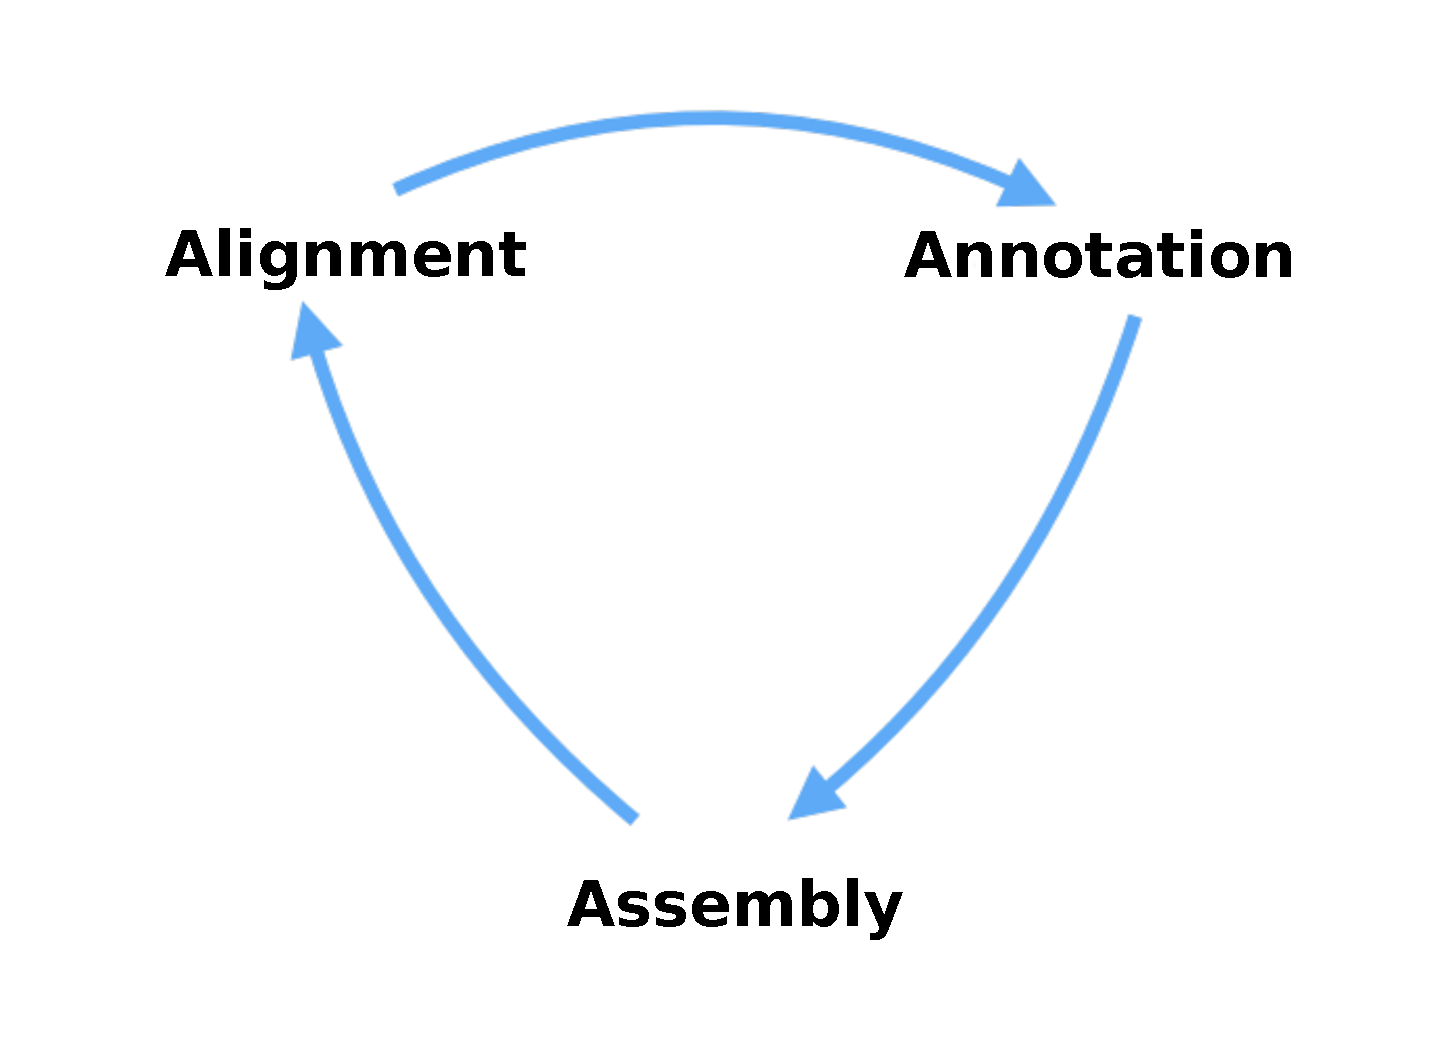
\includegraphics[scale=0.50]{images/three-As.pdf}}
  \only<2>{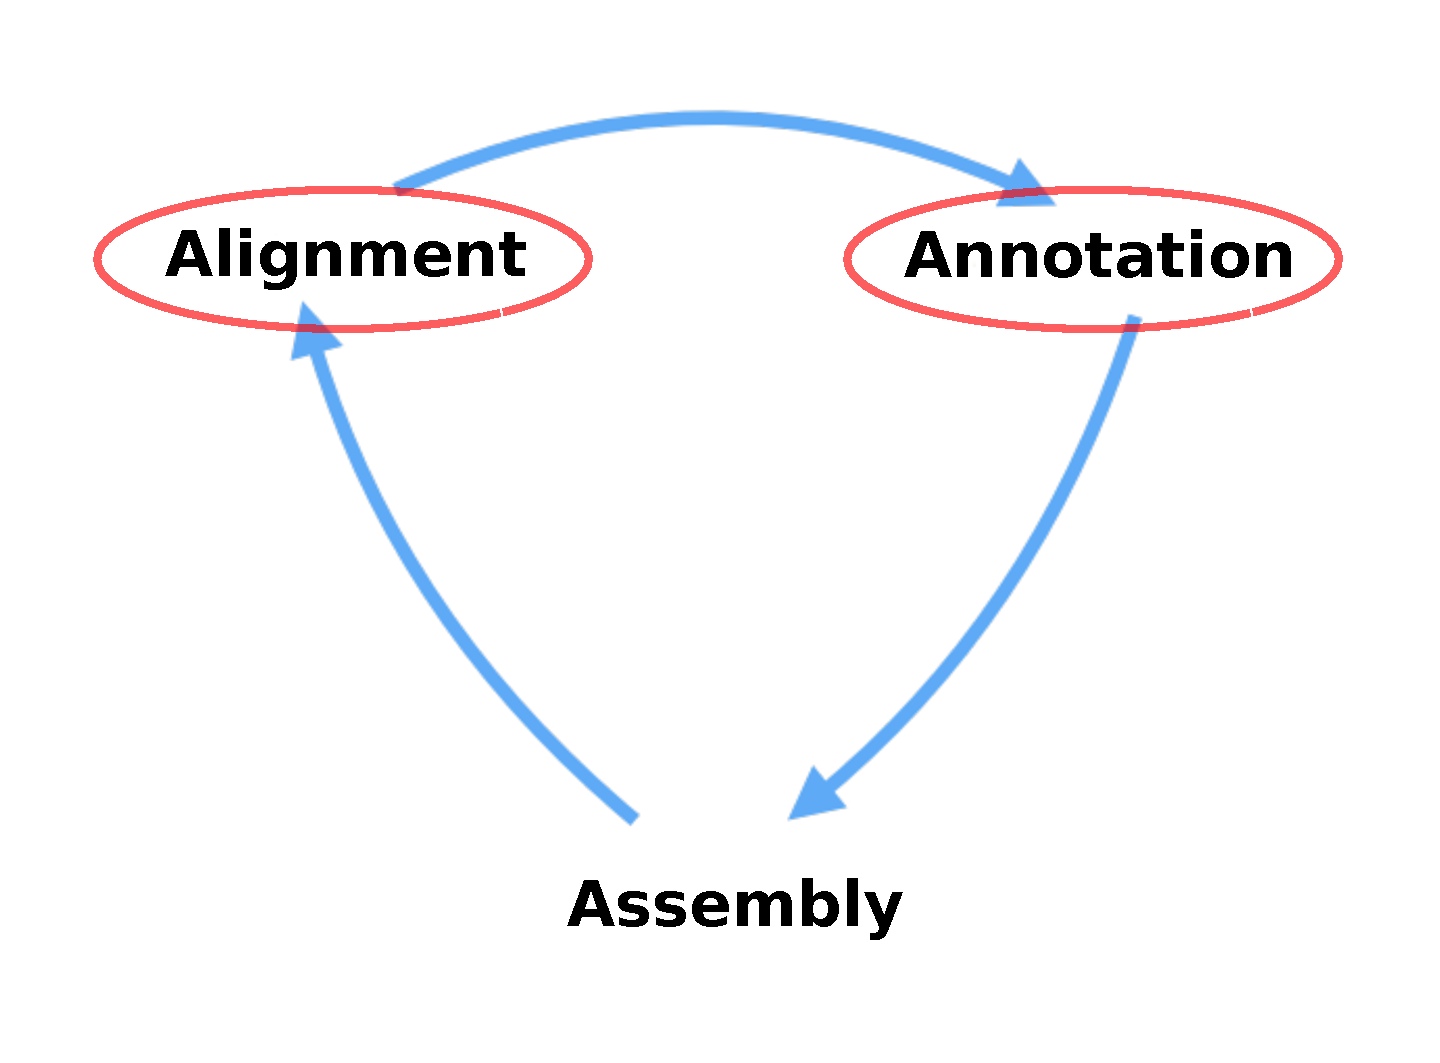
\includegraphics[scale=0.50]{images/our-two-As.pdf}}
\end{frame}


\begin{frame}{200 Mammals}
  \begin{columns}
    \begin{column}{0.5\textwidth}
      \begin{itemize}
          \item Extending earlier 29 Mammals project: from 29 mammals with 4.5 subs/site to 252 mammals with \char`~15 subs/site
          \item Generating 1bp-resolution constrained elements annotations
          \item Generating gene sets for all 252 assemblies using CAT
      \end{itemize}
    \end{column}
    \begin{column}{0.5\textwidth}
      \adjincludegraphics[trim={{0.2\width} 0 {0.2\width} 0},clip,width=\columnwidth]{images/200_Mammal_Tree.pdf}
    \end{column}
  \end{columns}
\end{frame}

\begin{frame}{Outline}
  \setbeamertemplate{section in toc}[sections numbered]
  \tableofcontents[hideallsubsections]
  \begin{itemize}
  \item Comparative genomics alignment
  \item Comparative genomics annotation
  \item Graph Genomes
  \item Transcript support
  \item UCSC Browser and GENCODE
  \end{itemize}
\end{frame}

\begin{frame}{Cactus}
  \begin{columns}
    \begin{column}{0.5\textwidth}
      \begin{itemize}
          \item Cactus is a non-reference-biased, whole-genome multiple-alignment tool
          \item Most genome multiple alignments are reference-biased: for any two non-reference genomes, any homologies between sequence not present in the reference are not aligned
          \item Reference-free alignments are harder to generate, but valuable for many comparative genomics applications
      \end{itemize}
    \end{column}
    \begin{column}{0.5\textwidth}
      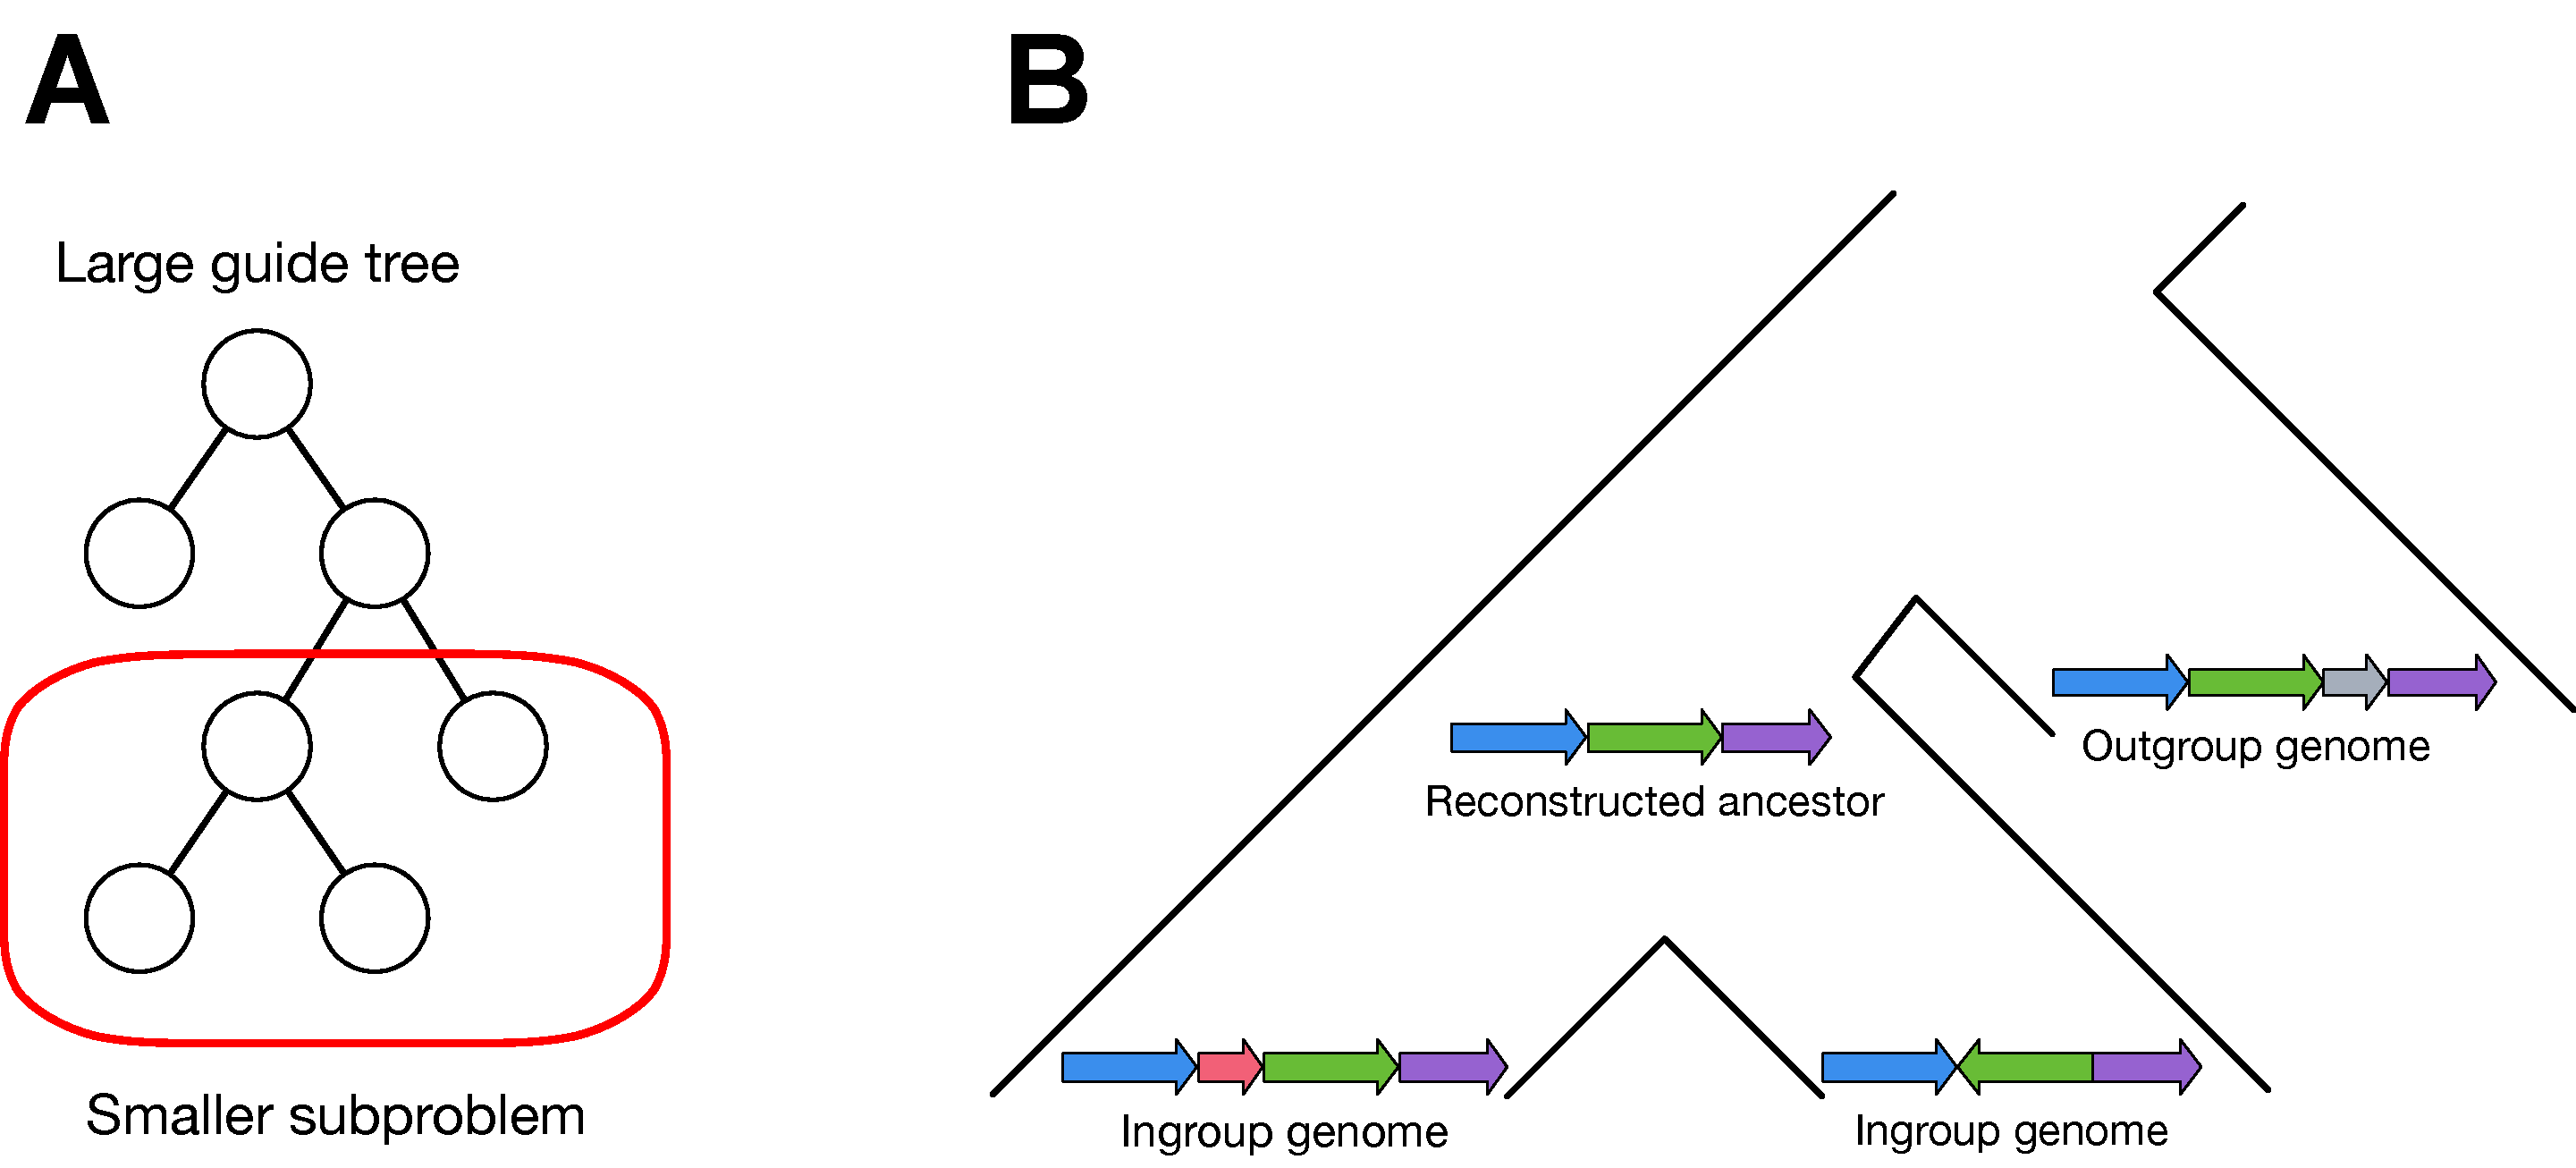
\includegraphics[width=\columnwidth]{images/progressive-alignment-and-reconstruction.pdf} \\
      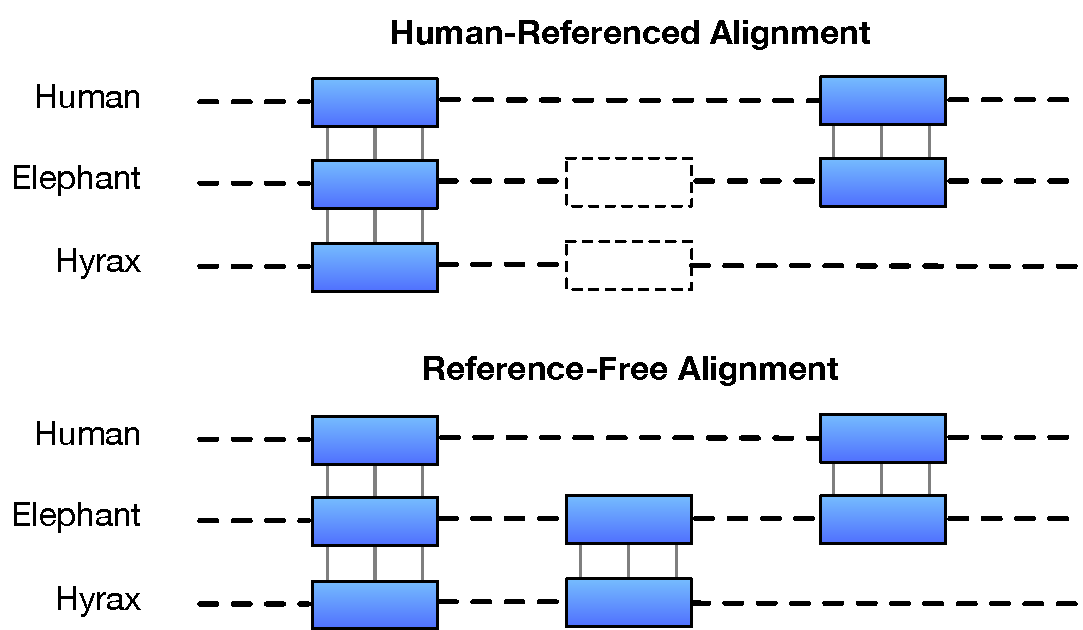
\includegraphics[width=\columnwidth]{images/reference-free-diagram.pdf}
    \end{column}
  \end{columns}
\end{frame}

\begin{frame}{RNA-Seq Intron Support}
  Goals:
  \begin{itemize}
  \item Evaluate support for 
  \end{itemize}
\end{frame}

\begin{frame}{RNA-Seq Intron Support}
  \centering
  \begin{itemize}
  \item CZI SRA alignments
  \item All SRA cloud run
  \item Array Express collaboration
  \end{itemize}
\end{frame}

\begin{frame}{RNA-Seq Intron Support}
  \begin{columns}
    \begin{column}{0.5\textwidth}
      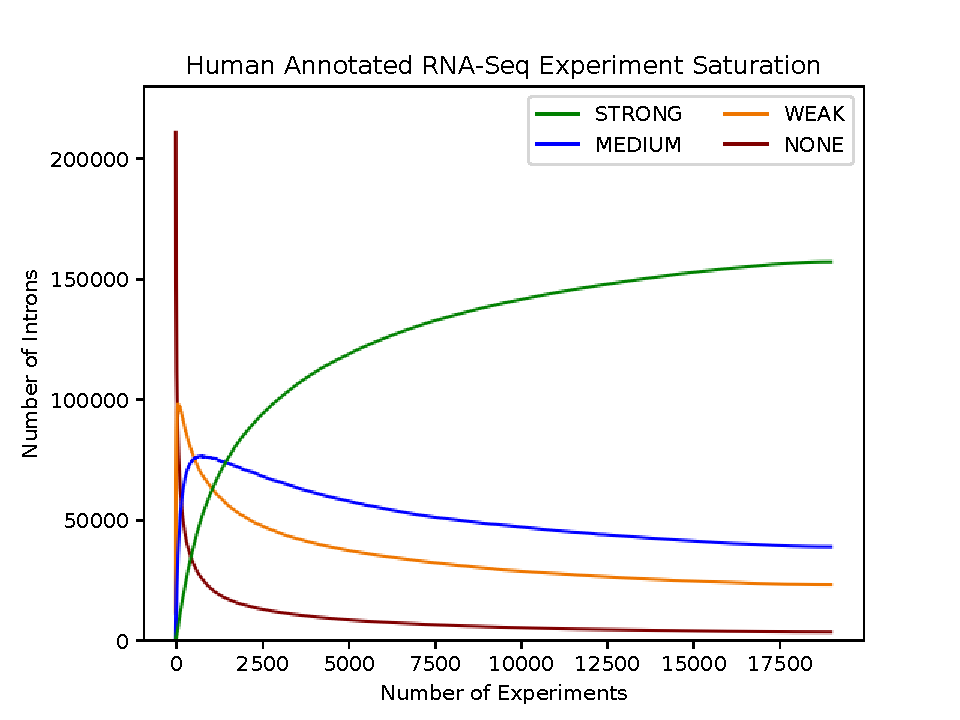
\includegraphics[scale=0.37]{images/hs_saturation_annot.pdf}
    \end{column}
    \begin{column}{0.5\textwidth}
      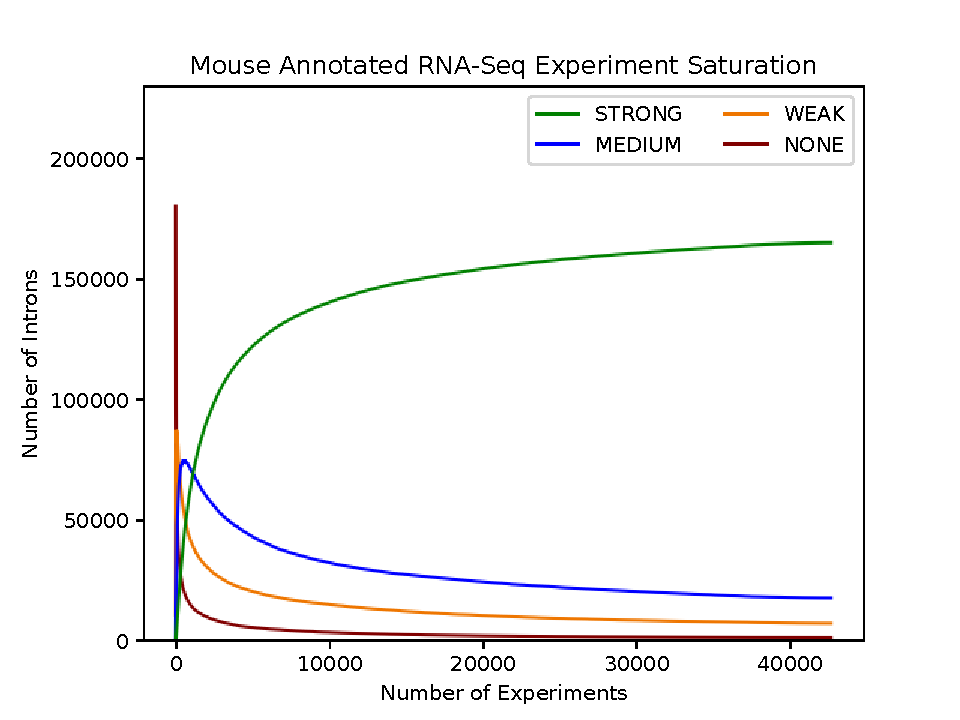
\includegraphics[scale=0.37]{images/mm_saturation_annot.pdf}
    \end{column}
  \end{columns}
  Experiment saturation for annotated introns
\end{frame}

\begin{frame}{RNA-Seq Intron Support}
  Working with Array Express
  \centering
  experiment and intron saturation
  
\end{frame}

\begin{frame}{RNA-Seq Intron Support}
  Approaches to Array Express integration
  \centering
  Splice junction calling external to ArrayExpress
  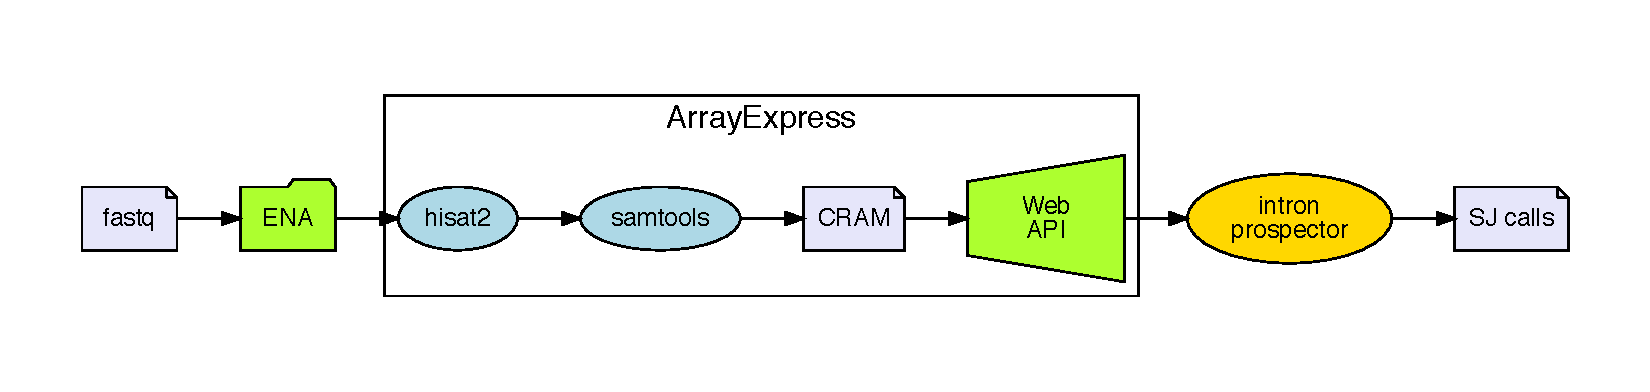
\includegraphics[scale=0.42]{images/calling_external.pdf}

  Splice junction calling in ArrayExpress RNA-Seq pipeline.
  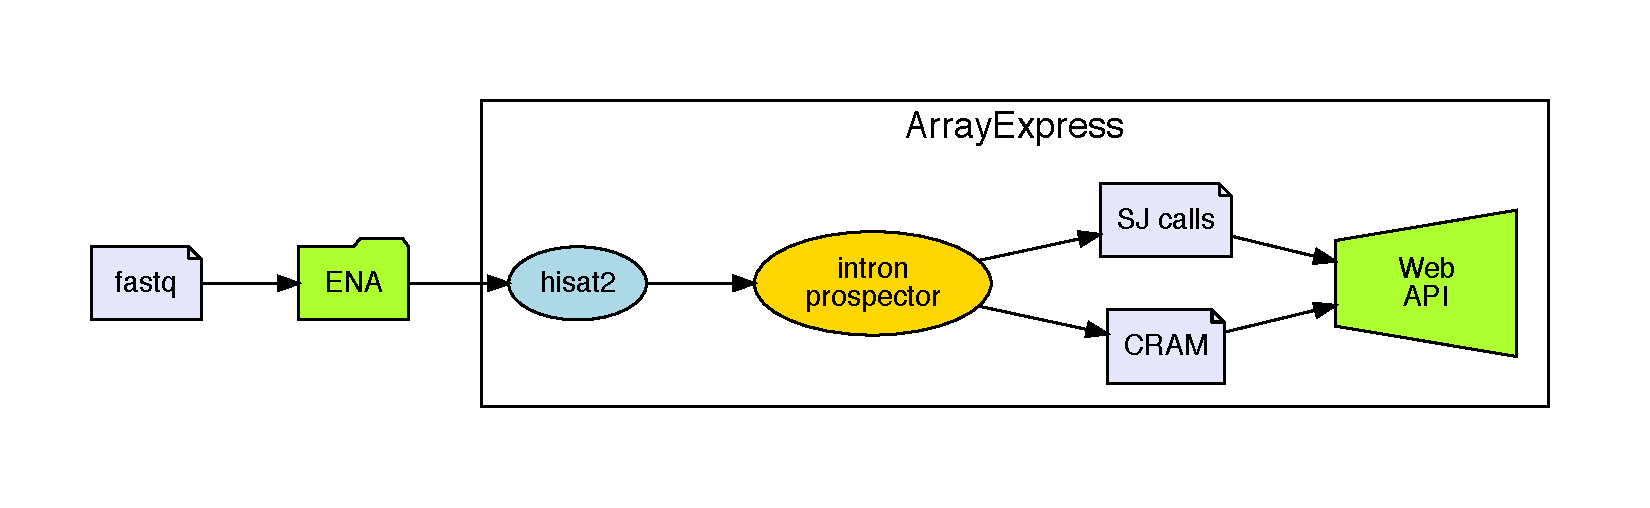
\includegraphics[scale=0.42]{images/calling_at_array_express.pdf}
\end{frame}

\iffalse
\begin{frame}{xxx}
  
  \centering
  \begin{itemize}
  \item zzz
  \end{itemize}
\end{frame}

\begin{frame}{}
  \centering
\end{frame}
\begin{frame}{}
  \centering
  \begin{itemize}
  \item 
  \end{itemize}
\end{frame}
\fi

\iffalse
- primate/CAT paper
\fi
\end{document}
